\part{Big-O-Notation}
\frame{\partpage}

\begin{frame}{What is Big 'O' Notation}
\begin{itemize}
	\pause \item The efficiency of an algorithm can be gauged by how long it takes
	\pause \item This is know as \textbf{Time Complexity}
	\pause \item \textbf{Big O Notation} is used to describe this
\end{itemize}
\end{frame}

\begin{frame}{Constant - O(1)}
	\begin{center}
		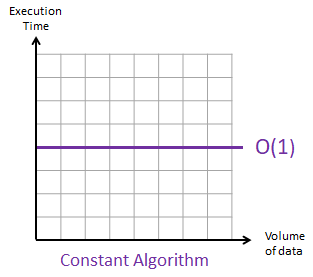
\includegraphics[height=0.8\textheight]{ConstantComplexity}
	\end{center}
\end{frame}

\begin{frame}{Linear - O(n)}
	\begin{center}
		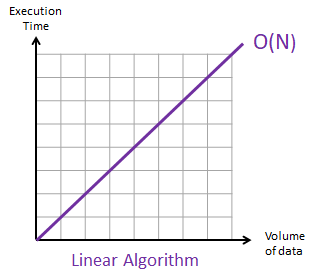
\includegraphics[height=0.8\textheight]{LinearComplexity}
	\end{center}
\end{frame}

\begin{frame}{Logarithmic - O(log(n))}
	\begin{center}
		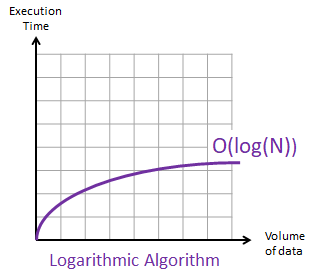
\includegraphics[height=0.8\textheight]{LogComplexity}
	\end{center}
\end{frame}

\begin{frame}{Big O Cheatsheet}
	\begin{center}
	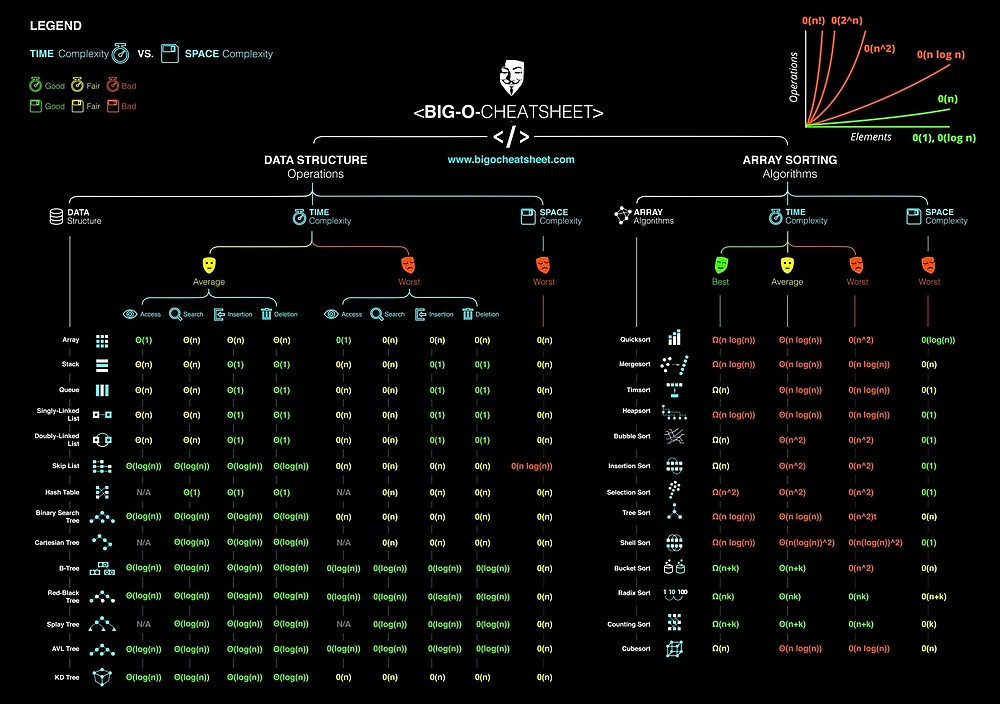
\includegraphics[height=0.8\textheight]{BigOCheatSheet}
	\end{center}
\end{frame}